
\documentclass[nooutcomes]{ximera}
%\documentclass[space,handout,nooutcomes]{ximera}

% For preamble materials

\usepackage{pgf,tikz}
\usepackage{mathrsfs}
\usetikzlibrary{arrows}
\usepackage{framed}
\usepackage{amsmath}
%\pgfplotsset{compat=1.16}

\graphicspath{
  {./}
  {algorithms/}
  {../algorithms/}
}

\pdfOnly{\renewenvironment{image}[1][]{\begin{center}}{\end{center}}}

%%% This set of code is all of our user defined commands
\newcommand{\bysame}{\mbox{\rule{3em}{.4pt}}\,}
\newcommand{\N}{\mathbb N}
\newcommand{\C}{\mathbb C}
\newcommand{\W}{\mathbb W}
\newcommand{\Z}{\mathbb Z}
\newcommand{\Q}{\mathbb Q}
\newcommand{\R}{\mathbb R}
\newcommand{\A}{\mathbb A}
\newcommand{\D}{\mathcal D}
\newcommand{\F}{\mathcal F}
\newcommand{\ph}{\varphi}
\newcommand{\ep}{\varepsilon}
\newcommand{\aph}{\alpha}
\newcommand{\QM}{\begin{center}{\huge\textbf{?}}\end{center}}

\renewcommand{\le}{\leqslant}
\renewcommand{\ge}{\geqslant}
\renewcommand{\a}{\wedge}
\renewcommand{\v}{\vee}
\renewcommand{\l}{\ell}
\newcommand{\mat}{\mathsf}
\renewcommand{\vec}{\mathbf}
\renewcommand{\subset}{\subseteq}
\renewcommand{\supset}{\supseteq}
\renewcommand{\emptyset}{\varnothing}
\newcommand{\xto}{\xrightarrow}
\renewcommand{\qedsymbol}{$\blacksquare$}
\newcommand{\bibname}{References and Further Reading}
\renewcommand{\bar}{\protect\overline}
\renewcommand{\hat}{\protect\widehat}
\renewcommand{\tilde}{\widetilde}
\newcommand{\tri}{\triangle}
\newcommand{\minipad}{\vspace{1ex}}
\newcommand{\leftexp}[2]{{\vphantom{#2}}^{#1}{#2}}

%% More user defined commands
\renewcommand{\epsilon}{\varepsilon}
\renewcommand{\theta}{\vartheta} %% only for kmath
\renewcommand{\l}{\ell}
\renewcommand{\d}{\, d}
\newcommand{\ddx}{\frac{d}{dx}}
\newcommand{\dydx}{\frac{dy}{dx}}


\usepackage{bigstrut}


\newenvironment{sectionOutcomes}{}{}

\usepackage{array}
%\setlength{\extrarowheight}{-.2cm}   % Commented out by Findell to fix table headings.  Was this for typesetting division?  
\newdimen\digitwidth
\settowidth\digitwidth{9}
\def~{\hspace{\digitwidth}}
\def\divrule#1#2{
\noalign{\moveright#1\digitwidth
\vbox{\hrule width#2\digitwidth}}}


\title{More Series}
\author{Bart Snapp and Brad Findell and Jenny Sheldon}
\begin{document}
\begin{abstract}
More problems about series.  Mostly geometric. 
\end{abstract}
\maketitle


%\begin{problem}
%Problem
%\begin{freeResponse}
%\begin{hint}
%Hint
%\end{hint}
%\end{freeResponse}
%\end{problem} 

\begin{problem}
A series is the $\answer[format=string]{sum}$ of consecutive terms from a(n) $\answer[format=string]{sequence}$.  

An arithmetic series is the $\answer[format=string]{sum}$ of consecutive terms from a(n) $\answer[format=string]{arithmetic sequence}$.  

A geometric series is the $\answer[format=string]{sum}$ of consecutive terms from a(n) $\answer[format=string]{geometric sequence}$.  
\end{problem}


\begin{problem}
Consider the geometric series: 
\[
\frac{1}{2}+\frac{1}{4}+\frac{1}{8}+\dots+\frac{1}{2048}
\]
First compute the sequence of partial sums: 
\[
\begin{array}{c|c} \hline
\text{No. of terms} & \text{Value} \\ \hline
1 & \answer{\frac{1}{2}} \\
2 & \answer{\frac{3}{4}} \\
3 & \answer{\frac{7}{8}}\\
4 & \answer{\frac{15}{16}}\\
5 & \answer{\frac{31}{32}}\\
6 & \answer{\frac{63}{64}}\\
\end{array}
\]
\begin{problem}
Make a conjecture: The sum of the first $n$ terms of this series is $\answer{1-\frac{1}{2^n}}$. 

In the series
\[
\frac{1}{2}+\frac{1}{4}+\frac{1}{8}+\dots+\frac{1}{2048}
\]
there are $\answer{11}$ terms, so the sum is $\answer{1-\frac{1}{2^{11}}}$.  

\begin{problem}

Here is picture that can help explain why this particular series works out so nicely: 
\begin{image}
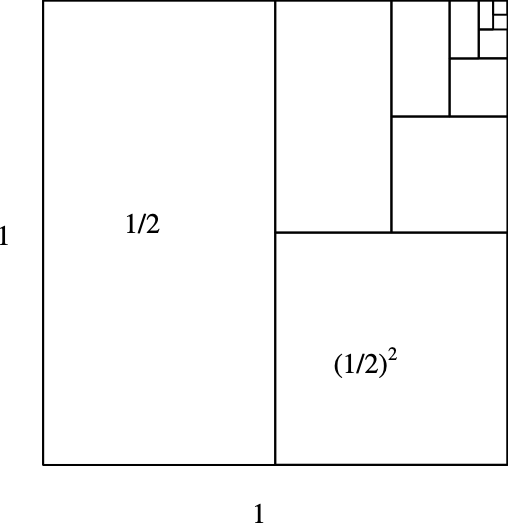
\includegraphics{pbpsqgeo.png}
\end{image}

Begin with a unit square, and then shade an area equal to each term.  At each step in the process, the area remaining unshaded is exactly equal to the area of the region last shaded.  For example, after shading $\frac{1}{2}$ and then $\frac{1}{4}$, 
$\answer{\frac{1}{4}}$ remains unshaded.  

Furthermore, it appears that as more and more terms are added, the sum should get closer and closer 
to $\answer{1}$.  

Here is GeoGebra sketch that allows you to explore similar series:  
%https://www.geogebra.org/m/tbheatqn
\begin{center}
\geogebra{tbheatqn}{720}{600}
\end{center}

The following problems demonstrate a general technique for geometric series.  

\begin{problem}
First, let 
\[
S=\frac{1}{2}+\frac{1}{4}+\frac{1}{8}+\dots+\frac{1}{2048}
\]
Multiply this equation by the common ratio $\answer{\frac{1}{2}}$ and place the two equations above/below one another so that identical terms align.  

\[
\begin{array}{ccccccccccccc}
                     S &=& \frac{1}{2} &+& \frac{1}{4} &+& \frac{1}{8} &+& \dots &+& \frac{1}{2048} \\ \\
\answer{\frac{S}{2}} &=&                & & \frac{1}{4} &+& \frac{1}{8} &+& \dots &+& \frac{1}{2048} 
         &+& \answer{\frac{1}{4096}}
\end{array}
\]
\begin{problem}
Then we $\answer[format=string]{subtract}$ the two equations so that most of the terms on the right vanish.  The result is a simpler equation: 
\[
S - \answer{\frac{S}{2}} = \frac{1}{2} - \answer{\frac{1}{4096}},
\]
which we can solve for $S$.  
\[
S = \frac{\frac{1}{2} - \answer{\frac{1}{4096}}}{1-\answer{\frac{1}{2}}},
\]
which simplifies to $S=\answer{1-\frac{1}{2^{11}}}$ as before.  
\begin{hint}
Remember to factor out the $S$ on the left before dividing.  
\end{hint}
\end{problem}
\end{problem}

\end{problem}
\end{problem}
\end{problem}



%\begin{problem}
%Use geometric series to explain how to convert repeating decimals to fractions to show they are rational numbers.  
%\begin{enumerate}
%\item  Express $0.232323...$ as geometric series.  Say how you know it is a geometric series.  Say also what it means to say it is an infinite geometric series.  
%\item  Find a closed expression (without decimals) for the exact sum of the first $n$ terms of the geometric series.  What decimal number does this represent?   
%\item  Explain what happens to that closed expression and to the decimal as $n$ increases to infinity. 
%\item  Explain what you may now conclude about the infinite decimal $0.232323...$.  
%\end{enumerate}
%\end{problem}
%


\begin{problem}
In this problem, we use geometric series to convert a repeating decimal to a fraction in order to show it 
is a $\answer[format=string]{rational}$ number.  

First express $0.\overline{23}=0.232323...$ as geometric series.  
\[
0.\overline{23}=\frac{23}{100}+\frac{23}{100^2}+\frac{23}{100^3}+\dots
\]
The series is geometric because the $\answer[format=string]{ratio}$ between consecutive terms is constant.  It equals $\answer{1/100}$.  

The series is infinite because to be \textbf{equal} to $0.\overline{23}$, we need to sum an infinite number of terms.  Any finite number of terms will be only a(n) $\answer[format=string]{approximation}$.  

\begin{problem}
To demonstrate the technique rigorously, we begin with a \textbf{finite} geometric series and find a closed expression (without decimals) for the exact sum.  

First, let 
\[
S=\frac{23}{100}+\frac{23}{100^2}+\frac{23}{100^3}+\dots+\frac{23}{100^n}
\]
Note that this is the finite decimal $0.2323 \dots 23$, with exactly $\answer{n}$ copies of the two repeating digits.  

We multiply this equation by the common ratio $\answer{1/100}$ and place the two equations above/below one another so that identical terms align.  

\[
\begin{array}{ccccccccccccc}
                     S &=& \frac{23}{100} &+& \frac{23}{100^2} &+& \frac{23}{100^3} &+& \dots &+& \frac{23}{100^n} \\ \\
\answer{\frac{S}{100}} &=&                & & \frac{23}{100^2} &+& \frac{23}{100^3} &+& \dots &+& \frac{23}{100^n} 
         &+& \answer{\frac{23}{100^{n+1}}}
\end{array}
\]
\begin{problem}
Then we $\answer[format=string]{subtract}$ the two equations so that most of the terms on the right vanish.  The result is a simpler equation: 
\[
S - \answer{\frac{S}{100}} = \frac{23}{100} - \answer{\frac{23}{100^{n+1}}},
\]
which we can solve for $S$.  
\[
S = \frac{\frac{23}{100} - \answer{\frac{23}{100^{n+1}}}}{1-\answer{\frac{1}{100}}}
\]
\begin{hint}
Remember to factor out the $S$ on the left before dividing.  
\end{hint}
\begin{problem}
As $n\rightarrow\infty$, $\frac{23}{100^{n+1}} \rightarrow\answer{0}$, so 
\[
S \rightarrow \frac{\answer{\frac{23}{100}}}{1-\frac{1}{100}}\text{, which simplifies to }\frac{\answer{23}}{\answer{99}}.
\]
From the original definition of $S$ above, when $n\rightarrow\infty$, we also have $S\rightarrow 0.\overline{23}$.  Therefore, 
\[
0.\overline{23}=\frac{\answer{23}}{\answer{99}},
\]
demonstrating that $0.\overline{23}$ is indeed a $\answer[format=string]{rational}$ number.  
\end{problem}
\end{problem}
\end{problem}
\end{problem}


\end{document}



